\documentclass{beamer}

\usepackage[czech]{babel}
\usepackage[utf8]{inputenc}
%\usepackage[plainpages=false,pdfpagelabels,unicode]{hyperref}
\usepackage{graphicx}

\usetheme{Warsaw}

\begin{document}

\title[Properties of DLC from optical measurements] % (optional, only for long titles)
{Properties of hydrogenated amorphous carbon films from optical measurements in wide spectral range}
\subtitle{The road so far...}
\author{Pavel Ondračka}
\institute
{
	 Faculty of Science, Masaryk University\\
	Brno, Czech Republic
  \and
	CEITEC - Central European Institute of Technology\\
	Brno, Czech Republic
}
\date{25.3.2015}

\maketitle

\begin{frame}
	\frametitle{Outline}
    \tableofcontents
\end{frame}

\section{Motivation}
\begin{frame}
    \frametitle{Motivation}
    \framesubtitle{You can measure almost everything with optics!}
	Optical measurements (ellipsometry, spectrophotometry) in broad spectral range are powerful techniques for thin film analysis.
	In theory we can obtain: 
	\begin{itemize}	
	\item optical constants (complex refractive index $\hat{n}$, dielectric function $\hat{\epsilon}$, absorbance, ...)
	\item structural properties of system (film thickness, roughness, inhomogenity, ...)
	\item information about electronic structure (carbon sp$^2$/sp$^3$ ratio)
	\item film density and composition
	\end{itemize}
	Hard hydrogenated amorphous carbon films (DLCH) should be a good test system. It is simple and we have a lot of samples.
\end{frame}

\section{Introduction}
\subsection{Hydrogenated amorphous carbon (a-C:H)}
\begin{frame}
    \frametitle{Why are DLCH interesting}
    \framesubtitle{Why is it so special?}
	\begin{columns}[c]
    \column{.4\textwidth}
	DLCH properties:
	\begin{itemize}
	\item high hardness
	\item excellent tribological properties
	\item bio-compatible
	\item easy to produce
	\end{itemize}

    \column{.6\textwidth}
    \begin{figure}
	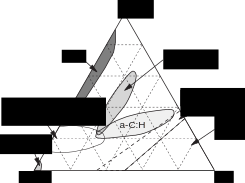
\includegraphics[width=\linewidth]{figures/DLCtypes.pdf}
	\end{figure}

	\end{columns}
\end{frame}

\subsection{Optics}
\begin{frame}
    \frametitle{Selected optical definitions}
    \framesubtitle{What all those letters stand for?}

	There are few terms to describe optical response:

	\begin{itemize}
	\item Refractive index $n$ and extinction coefficient $\kappa$, sometimes called complex refractive index $\hat{n} = n + \mathrm{i} \kappa$.
	\item Complex dielectric function $\hat{\epsilon} = \epsilon_\mathrm{r} + \epsilon_\mathrm{i}$, or for nonisotropic materials dielectric tensor $\hat{\epsilon}$.
	\item $\epsilon_\mathrm{r} = n^2 - \kappa^2 $, $\epsilon_\mathrm{i} = 2 n \kappa$
	\item Absorption (attenuation) coefficient $\alpha = \frac{4 \pi \kappa}{\lambda}$ as known from Beer-Lambert law $I = I_0 \mathrm{e}^{-\alpha x}$.
	\end{itemize} 
	\small
	\begin{equation}	
	\epsilon_\mathrm{i} (E) = 
\left(\frac{eh}{m_\mathrm{e}E} \right)^2 \frac{1}{4 \pi \epsilon_0 \mathrm{B}_0} \sum_{j,k} | p_{j \rightarrow k} |^2
\int_{-\infty}^\infty f_\mathrm{e}(S) \mathcal{N}_j(S) f_\mathrm{h}(S+E) \mathcal{N}_k(S + E)\mathrm{d}S \text{,}
	\end{equation}
	\normalsize
\end{frame}

\begin{frame}
    \frametitle{Selected optical definitions}
    \framesubtitle{No more equations, I promise}

Kramers-Kronig relations:
\begin{equation}
\epsilon_\mathrm{r}(\omega) = 1 + \frac{1}{\pi} \mathcal{P} \int \frac{\epsilon_\mathrm{i}(\xi)}{\xi - \omega} \mathrm{d}\xi \mathrm{.}
\label{KKint}
\end{equation}

So called optical sum rule:
\begin{equation}
\int_0^\infty \epsilon_\mathrm{i} (\omega) \omega \mathrm{d} \omega = \frac{\pi}{2} \omega_\mathrm{p}^2 = \frac{\pi}{2} \frac{e^2 n_\mathrm{e}}{ \epsilon_0 m_\mathrm{e}} \mathrm{.}
\end{equation}

\end{frame}

\section{Measurements}

\begin{frame}
   \frametitle{Available instruments}
   DLCH thin films were measured using following instruments:
	\begin{itemize}
	\item Bruker VERTEX 80v FTIR spectrofotometer (70--7500\,cm$^{-1}$)
	\item Jobin-Yvon UVISEL ellipsometer (0.56--6.5\,eV, variable angle of incidence)
	\item Jobin-Yvon UVISEL VUV ellipsometer (0.56--8.7\,eV)
	\item Perkin Elmer Lambda 1050 spectrophotometer (0.38--6.5\,eV)
	\item Elettra Sincrotrone Trieste - reflectance up to 50\,eV
	\end{itemize}
   Spectral range from FIR to VUV covers most of the interesting spectral regions.
\end{frame}

\section{Data analysis}
\subsection{Dispersion model}
\begin{frame}
    \frametitle{Dispersion model}
	\framesubtitle{The interesting stuff starts here...}
	\vspace{-0.2cm}
   \begin{itemize}
	\item To actually obtain some useful data, you need a suitable dispersion model.
	\item PJDOS-DLC dispersion model was developed based on models developed by Dr. Franta. 
	\item Total dielectric function is composed of contributions from different transition types $\hat{\epsilon}(E) = 1 + \sum_t \hat{\epsilon}_t(E)$
   \end{itemize} 
 
   \begin{figure}
   \begin{center}
	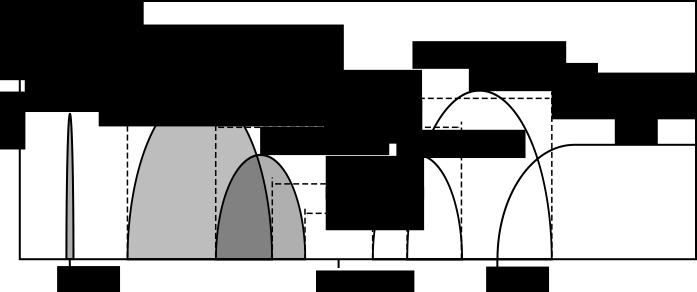
\includegraphics[width=0.75\linewidth]{figures/DLCDOS.pdf}
   \end{center}
	\end{figure}
   
\end{frame}

\subsection{Hydrogen content}
\begin{frame}
    \frametitle{Hydrogen content}
   \framesubtitle{This should be easy, it is the lightest element after all...}
	\begin{columns}[c]
    \column{.45\textwidth}
	\begin{itemize}
	\item Can be estimated from IR spectra, by fitting sp$^x$C-H$_y$ absorption peaks by gausians
   \item Unfortunately peaks are overlapping
   \item Different groups have different vibration strength
   \item To get relative concentration, density of carbon atoms is needed
   \end{itemize}

    \column{.55\textwidth}
	\begin{figure}
	\includegraphics[width=\linewidth]{figures/T-detail-multifit2.pdf}
	\end{figure}

   \end{columns}

\end{frame}

\begin{frame}
    \frametitle{Hydrogen content}
   \framesubtitle{Peaks everywhere!}

	\begin{figure}
	\includegraphics[width=0.5\linewidth]{figures/deconv-multifit2.pdf}
	\end{figure}

\end{frame}

\subsection{Mass density}
\begin{frame}
   \frametitle{Density}
   \framesubtitle{The basic ideas behind this}

   \begin{itemize}
	\item Electron density can be calculated from dielectric function.
	$$
	\int_0^\infty \epsilon_\mathrm{i} (\omega) \omega \mathrm{d} \omega = \frac{\pi}{2} \omega_\mathrm{p}	^2 = \frac{\pi}{2} \frac{e^2 n_\mathrm{e}}{ \epsilon_0 m_\mathrm{e}} \mathrm{,}
	$$
   \item Mass density can be calculated too, if we know composition.
   \item sp$2$/sp$3$ ratio can be deduced from ratio of $\sigma$ to $\pi$ electrons.
   \item sp$^3$C has 4 $\sigma$ electrons, sp$^2$ has 3 $\sigma$ and 1 $\pi$ electrons .
   \item However, hydrogen is also contributing $\sigma$ electrons.
   \end{itemize}

\end{frame}

\begin{frame}
   \frametitle{Density}
   \framesubtitle{Deconvolution of dielectric function}

	\begin{figure}
	\includegraphics[width=0.8\linewidth]{figures/CH30deconv.pdf}
	\end{figure}

\end{frame}


\begin{frame}
   \frametitle{Density}
   \framesubtitle{The sumrule strikes back}

   \begin{itemize}
	\item We need the whole spectra to calculate sumrule correctly.
   \item This is not possible.
   \item Partial sumrules over selected transitions does not hold, e.g. integrating over all valence electron transitions does not give you exact valence electron density.
   \item We can make it work with the concept of effective number of electrons.
   \item How to get the effective number of electrons? Ab-initio or calibrating with experimental results.
   \end{itemize}
\end{frame}

\begin{frame}
   \frametitle{Density calibration}
   \framesubtitle{Troubles with the ERDA/RBS}
	
	\begin{columns}[c]
    \column{.5\textwidth}
   \begin{itemize}
	\item Rutherford Back Scattering and Elastic Recoil Detection Analysis are commonly used tools to measure film density and composition.
   \item Nontrivial data evaluation - fitting is needed.
   \item Results are highly dependent on correct evaluation.
	\item Depending on method, relative hydrogen content can vary over 10\,\%!
   \end{itemize}
    \column{.5\textwidth}
	\begin{figure}
	\includegraphics[width=\linewidth]{figures/thickness.pdf}
	\end{figure}
   \end{columns}

\end{frame}

\begin{frame}
   \frametitle{Density results}
   \framesubtitle{It almost works... sort of}
	
   \begin{itemize}
	\item 4 samples were fitted in wide spectral region.
   \item Complicated model with roughness, inhomogeneity and transitional layer was needed.
   \item Hydrogen content was fixed to ERDA values.
   \item Problem with effective electron number was neglected.
   \end{itemize}
	\begin{table}
	\begin{tabular}{cccc}
	Sample & $f_\mathrm{H}$\,[\%] & $\rho$\,[g.cm$^{-3}$] & $\rho_{opt}$\,[g.cm$^{-3}$] \\ \hline \hline
	CH30M & 33 & 1.77 & 2.21\\
	CH83A & 49 & 1.31 & 1.96\\
	CH87A & 48 & 1.4 & 2.09\\
	CH88A & 38 & 1.6 & 2.21\\
	\end{tabular}
	\end{table}
\end{frame}

\section{Conclusions}
\begin{frame}
   \frametitle{Conclusions}
   \framesubtitle{How does the prospects look like}

   \begin{itemize}
	\item Obtaining mass density and hydrogen content from optics should be doable.
   \item Precise calibration method is crucial.
   \item Sample defects (roughness, inhomogeneity, etc.) can influence results a lot.
	\item Ab-initio computations can help.
	\item Even with everything working, the method precision might not be best due to correlation.
   \end{itemize}
   %\end{columns}

\end{frame}

\begin{frame}
    \frametitle{Questions}
    \framesubtitle{Everything was clear, wasn't it?}

	\begin{center}
	Thank you for your attention.
	\end{center}
	\begin{center}
	Time for questions!
	\end{center}

\end{frame}

\end{document}
